% KU Leuven latex presentation template
%
% © 2012 Michael Hofmann
%
% This work is licensed under the Creative Commons Attribution 3.0 Unported License.
% To view a copy of this license, visit
% http://creativecommons.org/licenses/by/3.0/ or send a letter to Creative
% Commons, 444 Castro Street, Suite 900, Mountain View, California, 94041, USA.

\documentclass[t,12pt,english
\ifx\beamermode\undefined\else,\beamermode\fi
]{beamer}
%\setbeameroption{show notes}
%\setbeameroption{show only notes}
%\usepackage{caption}
\usepackage[utf8]{inputenc}
\usepackage[T1]{fontenc}
\usepackage{amsmath}
\usepackage[nohyperlinks]{acronym}
\usepackage{babel,lmodern,graphicx,mathptmx,xspace,wasysym,microtype,booktabs,tabularx,relsize,textcomp,longtable,lipsum,colortbl,eurosym,url,multicol,etoolbox,multimedia,pdfpages,fixltx2e,ifluatex,epstopdf}
\usepackage[olditem,oldenum]{paralist}
\usepackage[babel=true]{csquotes}
\usepackage[thinqspace,amssymb,textstyle]{SIunits}
\usepackage[textsize=tiny]{todonotes}
\usepackage[symbol]{footmisc}
\usepackage[notquote]{hanging}
\usepackage[normalem]{ulem}
%\usepackage{lua-visual-debug}

\pdfstringdefDisableCommands{\renewcommand{\sout}{}}
\graphicspath{{Session1/}}
% Fix sort order in case the same file exists with multiple extensions
\DeclareGraphicsExtensions{.pdf,.png,.jpeg,.jpg,.eps}
\frenchspacing

\input{templates/definitions.tex}



%% From pandoc default template
%% End pandoc

\mode<presentation>

%\hypersetup{pdfpagemode=FullScreen}

\definecolor{kuldefault}{HTML}{00407a}
\definecolor{kulbright}{HTML}{52bdec}
\definecolor{kulleft}{HTML}{1d8db0}
\definecolor{kulright}{HTML}{116e8a}

\definecolor{kulyellow}{HTML}{BC8F00}
\definecolor{kulorange}{HTML}{BC6E00}
\definecolor{kulgreen}{HTML}{007F4F}
\definecolor{kulred}{HTML}{FF4422}

\setbeamercolor{structure}{fg=kulbright}
\setbeamercolor{title}{fg=white}
\setbeamercolor{footline}{parent=title}
\setbeamercolor{normal text}{fg=kuldefault}
\setbeamercolor{item}{parent=normal text}
\setbeamercolor{section in toc}{parent=normal text}
\setbeamerfont{title}{size=\Large}
\setbeamerfont{tiny structure}{series=\bfseries}
\setbeamerfont{caption}{}

\setbeamersize{text margin left=0.8cm}
\setbeamersize{text margin right=0.8cm}
\setbeamersize{sidebar width left=0cm}

\setbeamertemplate{navigation symbols}{}
\setbeamertemplate{itemize item}{\footnotesize\raise1pt\hbox{\textbullet}}
\setbeamertemplate{itemize subitem}{--}
\setbeamertemplate{itemize subsubitem}{\tiny\raise1.5pt\hbox{\textbullet}}

\setlength\leftmargini{1em}
\setlength\leftmarginii{1em}
\setlength\leftmarginiii{1em}

\defbeamertemplate{background canvas}{title}
{%
    \pgfdeclarehorizontalshading{bgshading}{8.70cm}{color(0cm)=(kulleft); color(\the\paperwidth)=(kulright)}%
    \vbox to 8.70cm{%
        \pgfuseshading{bgshading}\hspace*{-1.6cm}%
    }%
    \hskip-\paperwidth%
    \hskip1.6cm%
    \vbox to \paperheight{%
        \vskip0.5cm\hskip0.5cm\includegraphics[width=2.83cm]{templates/kuleuven}%
        \vskip0.99cm\hskip0.76cm\includegraphics[width=2.84cm]{templates/key}%
        \vskip-0.57cm\hskip11.61cm\includegraphics[width=0.58cm]{templates/sedes}\hspace*{-1cm}%
        \vfill
    }%
}

\defbeamertemplate{background canvas}{grid}
{%
    \begin{tikzpicture}[remember picture,overlay,every node/.style={anchor=center}]
        \foreach \d in {0,...,20} {
            \draw[gray] (\d,0) -- (\d,-20);
            \draw[gray] (0,-\d) -- (20,-\d);
            \draw[lightgray] (\d+0.5,0) -- (\d+0.5,-20);
            \draw[lightgray] (0,-\d-0.5) -- (20,-\d-0.5);
            \node[anchor=north,red,font=\tiny] at (\d,0) {\d};
            \node[anchor=west,red,font=\tiny] at (0,-\d) {\d};
        }
    \end{tikzpicture}
}

\defbeamertemplate{background canvas}{plain}{}

\defbeamertemplate{footline}{large}
{%
    \pgfdeclarehorizontalshading{bgshading}{0.62cm}{color(0cm)=(kulleft); color(\the\paperwidth)=(kulright)}%
    \vskip.3cm% make room for the logo
    \parbox[t][0.62cm]{\paperwidth}{\pgfuseshading{bgshading}}\par%
    \vskip-0.62cm%
    \begin{beamercolorbox}[ht=0.37cm,dp=0.25cm,center]{page number in head/foot}%
    \insertframenumber%
    \end{beamercolorbox}%
    \vskip-0.92cm%
    \parbox[t][0.92cm]{\paperwidth}{\hskip10.33cm\includegraphics[width=2.10cm]{templates/kuleuven}}\par%
}

\defbeamertemplate{footline}{nopagenumber}
{%
    \pgfdeclarehorizontalshading{bgshading}{0.62cm}{color(0cm)=(kulleft); color(\the\paperwidth)=(kulright)}%
    \vskip.3cm% make room for the logo
    \parbox[t][0.62cm]{\paperwidth}{\pgfuseshading{bgshading}}\par%
    \vskip-0.62cm%
    \begin{beamercolorbox}[ht=0.37cm,dp=0.25cm,center,ignorebg]{page number in head/foot}%
    %
    \end{beamercolorbox}%
    \vskip-0.92cm%
    \parbox[t][0.92cm]{\paperwidth}{\hskip10.33cm\includegraphics[width=2.10cm]{templates/kuleuven}}\par%
}

\defbeamertemplate{footline}{small}
{%
    \vskip.3cm% make room for the logo
    \begin{beamercolorbox}[ht=0.37cm,dp=0.25cm,center,ignorebg]{normal text}%
    \mdseries\insertframenumber%
    \end{beamercolorbox}%
}

\setbeamertemplate{footline}[large]

\setbeamertemplate{frametitle}
{%
    \nointerlineskip%
    \vskip.28cm%
    {\usebeamercolor[fg]{framesubtitle}\usebeamerfont{framesubtitle}\insertsupertitle\strut\par}%
    \vskip-.2cm%
    {\usebeamercolor[fg]{frametitle}\usebeamerfont{frametitle}\insertframetitle\strut\par}%
    \vskip-.3cm%
}

\setbeamertemplate{title page}
{
    \vbox{}%
    \vskip2.8cm%
    \vbox to 6.5cm{%
        \hskip2.8cm%
        \begin{minipage}{7.9cm}
            \begin{beamercolorbox}{title}
                \usebeamerfont{title}%
                \inserttitle\par%
                \ifx\insertsubtitle\undefined%
                \else%
                    \vskip0.25em%
                    {\usebeamerfont{subtitle}\usebeamercolor[fg]{subtitle}\insertsubtitle\par}%
                \fi%
            \end{beamercolorbox}%
            \vskip1em\par
            \begin{beamercolorbox}{author}
                \usebeamerfont{author}\usebeamercolor[fg]{subtitle}%
                \insertauthor
            \end{beamercolorbox}
            \begin{beamercolorbox}{institute}
                \usebeamerfont{institute}\usebeamercolor[fg]{subtitle}%
                \insertinstitute
                \end{beamercolorbox}
            \begin{beamercolorbox}{date}
                \usebeamerfont{date}\usebeamercolor[fg]{subtitle}%
                \insertdate
            \end{beamercolorbox}%
        \end{minipage}%
        \vfill
    }
}

\mode<all>

\newcommand{\inlinesound}[2]{\movie[inlinesound,encoding=Signed,samplingrate=44100]{#1}{#2}}

% disable for now as otherwise all commands that go between frames generated by
% the filter will result in duplicate toc lines
\renewcommand{\addcontentsline}[3]{}

\newcommand{\largefooter}{\setbeamertemplate{footline}[large]}
\newcommand{\emptyfooter}{\setbeamertemplate{footline}[nopagenumber]}
\newcommand{\smallfooter}{\setbeamertemplate{footline}[small]}

\newcommand{\sectiontoc}{\AtBeginSection[]{{
    \nosupertitle
    \emptyfooter
    \begin{frame}[noframenumbering]{Outline}
                \tableofcontents[currentsection]
            \end{frame}
    \largefooter
}}}

\newcommand{\subsectiontoc}{\AtBeginSubsection[]{{
    \nosupertitle
    \emptyfooter
    \begin{frame}[noframenumbering]{Outline}
                \tableofcontents[currentsection,currentsubsection]
           \end{frame}
    \largefooter
}}}

\newcommand{\notoc}{\AtBeginSection[]{}\AtBeginSubsection[]{}}

\newcommand{\nosupertitle}{\renewcommand{\insertsupertitle}{}}
\newcommand{\sectiontitle}{\renewcommand{\insertsupertitle}{\insertsectionhead}}
\newcommand{\subsectiontitle}{\renewcommand{\insertsupertitle}{\insertsectionhead\ifx\insertsubsectionhead\empty\else{} -- \insertsubsectionhead\fi}}

% animations do not work atm as figures are set on independent frames
\newcommand{\slidefig}[2]{\usebackgroundtemplate{\parbox[c][\paperheight][c]{\paperwidth}{\centering\includegraphics#1[height=\paperheight,width=\paperwidth,keepaspectratio]{#2}}}\begin{frame}[plain]\end{frame}\usedefaultcanvas}

\newcommand{\usedefaultcanvas}{\setbeamertemplate{background canvas}[\defaultcanvas]}
\newcommand{\gridcanvas}{\renewcommand{\defaultcanvas}{grid}\usedefaultcanvas}
\newcommand{\plaincanvas}{\renewcommand{\defaultcanvas}{plain}\usedefaultcanvas}

\newcommand{\insertsupertitle}{}






\newcommand{\defaultcanvas}{plain}


% Defining a new coordinate system for the page:
%
% ----------------
% |(0,1)    (1,1)|
% |              |
% |(0,0)    (1,0)|
% ----------------
\makeatletter
\def\parsecomma#1,#2\endparsecomma{\def\page@x{#1}\def\page@y{#2}}
\tikzdeclarecoordinatesystem{page}{
    \parsecomma#1\endparsecomma
    \pgfpointanchor{current page}{north east}
    % Save the upper right corner
    \pgf@xc=\pgf@x%
    \pgf@yc=\pgf@y%
    % save the lower left corner
    \pgfpointanchor{current page}{south west}
    \pgf@xb=\pgf@x%
    \pgf@yb=\pgf@y%
    % Transform to the correct placement
    \pgfmathparse{(\pgf@xc-\pgf@xb)*\page@x+(\pgf@xb)}
    \expandafter\pgf@x\expandafter=\pgfmathresult pt
    \pgfmathparse{(\pgf@yc-\pgf@yb)*\page@y+(\pgf@yb)}
    \expandafter\pgf@y\expandafter=\pgfmathresult pt
}
\makeatother

% Example:
%\begin{tikzpicture}[remember picture,overlay,every node/.style={anchor=center}]
%  \node at (page cs:0.5,0.3) {0.5,0.3};
%  \node at (page cs:0,0) {0,0};
%  \draw(page cs:0,0) -- (page cs:1,1);
%  \draw[thick,red] (page cs:0,0) rectangle (page cs:1,1);
%  \draw[thick,green] (page cs:0.2,0.2) rectangle (page cs:0.8,0.8);
%\end{tikzpicture}

\setcounter{secnumdepth}{0}

\title{Subspace Signal Processing}
\subtitle{\tiny Biomedical Data Procession part II}
\author{\\ \href{vangjush.komini@uzleuven.be}{\textbf{\textit{Vangjush Komini}}}
}


\institute{{\tiny }\vspace{.10cm} }
\date{\href{www.kul.be}{KU Leuven}\\ \vspace{.10cm}\today}

\begin{document}

\setbeamertemplate{background canvas}[title]

\begin{frame}[plain,noframenumbering]
    \titlepage
\end{frame}

\usedefaultcanvas


\emptyfooter
\begin{frame}[noframenumbering]{Outline}
        \tableofcontents
    \end{frame}
\largefooter

\section{Artifact removal}\label{first-section}

\begin{frame}{Artifact removal}
   
   

\begin{figure}[!htbp]
\minipage{.5\textwidth}%
\centering
\includegraphics[width=.8\textwidth]{1.jpg}
\caption{\tiny Acquire signal in time domain}\label{1}
\endminipage\hfill
\minipage{.5\textwidth}%
\centering
\includegraphics[width=.8\textwidth]{2.jpg}
\tiny\caption{\tiny Spectrum of the signal in ppm}\label{2}
\endminipage\hfill
\end{figure}

 

\begin{equation}
ppm=\frac{f_{Hz}*10^6}{f_{s}}-ppm_{Ref}
\end{equation}
    

\begin{equation}\label{eq1}
y(t)=\sum_{k=1}^{K} a_{k}exp(j\phi_{k})exp(-d_{k}t+2\pi f_{k}t)\delta t
\end{equation}
   
\end{frame}

\begin{frame}{Decomposition of the component}

\begin{figure}[!htbp]
\centering
\includegraphics[width=1\textwidth]{5.jpg}
\caption{\tiny{Spectrum of decomposed components }}
\end{figure}

\end{frame}

\begin{frame}{Decomposition of the component}

\begin{figure}[!htbp]
\centering
\includegraphics[width=1\textwidth]{6.jpg}
\caption{\tiny{Components in time domain}}
\end{figure}
    
\end{frame}

\begin{frame}{Filtering of the signal}
\begin{figure}[!htbp]
\centering
\includegraphics[width=1\textwidth]{8_2.jpg}
\caption{\tiny{Filtering of the MRS spectrum for different model order}}
\end{figure}   
\end{frame}

\begin{frame}{Filtering of the signal}
\begin{figure}[!htbp]
\centering
\includegraphics[width=1\textwidth]{8.jpg}
\caption{\tiny{Filtering of the MRS spectrum for different model order}}
\end{figure}   
\end{frame}

\begin{frame}{Over view of the performance}

\begin{figure}[!htbp]
\minipage{.5\textwidth}%
\centering
\includegraphics[width=1\textwidth]{8_1.jpg}\\
\tiny{Spectrum Water filtered signal for model order 30}\label{fig2}
\endminipage\hfill
\minipage{.5\textwidth}%
\centering
\includegraphics[width=1\textwidth]{11.jpg}\\
\tiny{Signal-to-noise ration for different model order estimation}\\
\endminipage\hfill
\end{figure}

\begin{equation}
SNR=20*\log\bigg\{\frac{OriginalSignal}{FilteredSignal-OriginalSignal}\bigg\}
\end{equation} 

\end{frame}


\begin{frame}{Comparison with classical filters}

\begin{block}{\footnotesize{}}\tiny{}
\begin{enumerate} 
\vspace{0.05cm}
     \item \tiny{\textbf{\textit{Spectral method are FFT based $O(nlog(n))$ vs SVD based $O(nm^2)$}}}
     \item \tiny{\textbf{\textit{Minimal distortion of the wanted signal and better noise reduction}}}
     \item \tiny{\textbf{\textit{A clear analytical formulation of the problem is needed for the subspace case}}} 
     \item \tiny{\textbf{\textit{Difficult but still possible incorporation of prior knowledge in subspace}}} 
%     \item \tiny{\textbf{\textit{DCT is another competitive apart from FFt yet, far inferior compare to subspace filtering}}} 

     
\end{enumerate}
\end{block}
  
\end{frame}

\section{Parameter estimation}\label{second-section}

\begin{frame}{Parameter estimation}
    
\begin{figure}[!htbp]
\minipage{.47\textwidth}%
\centering
\includegraphics[width=1\textwidth]{35.jpg}
\caption{\tiny Spectrum of signals to be processed}
\endminipage\hfill
\minipage{.47\textwidth}%
\centering
\includegraphics[width=1\textwidth]{36.jpg}
\caption{\tiny The signals to be processed in time domain}
\endminipage\hfill
\centering
\end{figure}

\tiny{The pure water filtered signal at model order 30 and the noisy signal coming from the superposition of the white Gaussian noise with mean zeros and the variance equal last 300 points of the water filtered signal}  

\end{frame}


\begin{frame}{Reconstructed signal}

\begin{figure}[!htbp]
\minipage{.47\textwidth}%
\centering
\includegraphics[width=1\textwidth]{22.jpg}
\caption{\tiny Reconstruction of noise free signal after hsvD, htls, htlspk estimation}\label{today1}
\endminipage\hfill
\minipage{.47\textwidth}%
\centering
\includegraphics[width=1\textwidth]{23.jpg}
\caption{\tiny Reconstruction of noisy signal after hsvD, htls, htlspk estimation}\label{today2}
\endminipage\hfill
\end{figure}
\tiny{Plot of the reconstructed spectrum for both the  pure and noisy signal}
    
\end{frame}

\begin{frame}{Fitting error}


\begin{figure}[!htbp]
\minipage{.47\textwidth}%
\centering
\includegraphics[width=1\textwidth]{24.jpg}
\caption{\tiny Residue of noise free signal after hsvD, htls, htlspk estimation}
\endminipage\hfill
\minipage{.47\textwidth}%
\centering
\includegraphics[width=1\textwidth]{25.jpg}
\caption{\tiny Residue of noisy signal after hsvD, htls, htlspk estimation}
\endminipage\hfill
\centering
\end{figure}

\tiny{The residue of both pure and noisy signals are included. This is computed as the difference between the input signal \textit{(pure or noisy)} and the outcome signal for respective method.}

\end{frame}

\begin{frame}{Parameter estimation}


\begin{figure}[!htbp]
\minipage{.5\textwidth}%
\centering
\includegraphics[width=.8\textwidth]{12.jpg}

\endminipage\hfill
\minipage{.5\textwidth}%
\centering
\includegraphics[width=.8\textwidth]{13.jpg}
\endminipage\hfill
\minipage{.5\textwidth}%
\centering
\includegraphics[width=.8\textwidth]{14.jpg}
\endminipage\hfill
\minipage{.5\textwidth}%
\centering
\includegraphics[width=.8\textwidth]{15.jpg}
\endminipage\hfill
\end{figure}
    
\end{frame}


\begin{frame}{Subspaces method for parameter estimation}
 

\begin{block}{\footnotesize{}}\tiny{}
\begin{enumerate} 
\vspace{0.05cm}
      
     \item \tiny{\textbf{\textit{Bias method for estimation of parameters}}} 
     \item \tiny{\textbf{\textit{CR lower bound is reduced by incorporating prior knowledge}}} 
     \item \tiny{\textbf{\textit{Robust estimation of the parameters}}}
     \item \tiny{\textbf{\textit{Subspace methods are very good candidate for the parameter estimation of closely spaced sinusoid}}} 
     \item \tiny{\textbf{\textit{The user capability to initialize the parameters of the subspace methods is very important}}} 
     \item \tiny{\textbf{\textit{It ensures the best estimation outside the local minimum}}} 
     \item \tiny{\textbf{\textit{Capable of estimation multiple parameter at the same time instead of ALS solution}}} 
     \item \tiny{\textbf{\textit{Does not ensure the reproducibility of the parameters}}} 
     
\end{enumerate}
\end{block}
    
\end{frame}


\section{Noise reduction}\label{third-section}

\begin{frame}{Noise reduction}
   
\begin{figure}[!htbp]
\minipage{.47\textwidth}%
\centering
\includegraphics[width=1\textwidth]{27.jpg}
\caption{\tiny Original signal and its respective enhancement after Cadzow, Minimum variance, Multichannel Cadzow, and Enhanced Multichannel Cadzow}
\endminipage\hfill
\minipage{.47\textwidth}%
\centering
\includegraphics[width=1\textwidth]{28.jpg}
\caption{\tiny Original signal and its respective estimation after Cadzow, Minimum variance, Multichannel Cadzow, and Enhanced Multichannel Cadzow enhancement}
\endminipage\hfill
\end{figure}

\end{frame}

\begin{frame}{Performance evaluation}

\begin{table}[!htbp]
\centering
\label{table:55}
\begin{tabular}{c c c c c c c c c c c c c c c c c}
$Method$&$SNR(dB)$\\
  \hline  
$Filtered signal$&$-25.2546$\\
$Cadzow$&$3.7264$\\
$MinimVariance$&$3.7270$\\
$MultiChannel$&$39.5513$\\
$OptimMultiChannel$&$40.1137$\\
  \hline  
\end{tabular}
\end{table}  

{The best performance is achieved with vertically and horizontally neighbours at order of 22 with 3x3 voxels} 
     
\end{frame}

\begin{frame}{Multichannel voxels}
    
\begin{figure}[!htbp]
\centering
\includegraphics[width=1\textwidth]{37.jpg}
\caption{\tiny 9x9 voxel neighbourhood with the voxel of interest in the middle}\label{figtoda1}
\end{figure}

\end{frame}


\begin{frame}{Parameter estimation via HTLS method}

\begin{figure}[!htbp]
\minipage{.5\textwidth}%
\centering
\includegraphics[width=.8\textwidth]{31.jpg}
\endminipage\hfill
\minipage{.5\textwidth}%
\centering
\includegraphics[width=.8\textwidth]{32.jpg}
\endminipage\hfill
\minipage{.5\textwidth}%
\centering
\includegraphics[width=.8\textwidth]{33.jpg}
\endminipage\hfill
\minipage{.5\textwidth}%
\centering
\includegraphics[width=.8\textwidth]{34.jpg}
\endminipage\hfill
\end{figure}

\end{frame}

\begin{frame}{Cadzow vs Minimum Variance}

\begin{block}{\footnotesize{}}\tiny{}
\begin{enumerate} 
\vspace{0.05cm}
     
    \item \tiny{\textbf{\textit{Minimum Variance algorithm significantly improves the frequency resolution.}}}
    \item \tiny{\textbf{\textit{Differences of estimation of the parameters for the peaks are relatively small.}}}
    \item \tiny{\textbf{\textit{An overestimate model will not increase the accuracy.}}}
    \item \tiny{\textbf{\textit{MV aims to minimize the variance it will outcome an overall improved performance.}}}
    \item \tiny{\textbf{\textit{Algorithm is not limited into white noise contamination}}}
    \item \tiny{\textbf{\textit{Proportionally to the number of data points and model order it is possible to double the resolution irrespectively to the noise variance. }}}
     
\end{enumerate}
\end{block}

\end{frame}

\begin{frame}{Cadzow vs Multi-Channel Cadzow}

\begin{block}{\footnotesize{Cadzow vs Multi-Channel Cadzow}}\tiny{}
\begin{enumerate} 
\vspace{0.05cm}
    \item \tiny{\textbf{\textit{Cadzow perform blindly from the further voxels.}}}
    \item \tiny{\textbf{\textit{Correlation between the channels can be fully exploited.}}}
    \item \tiny{\textbf{\textit{Better interpolation of information from the surrounding is performed.}}}
    \item \tiny{\textbf{\textit{Unwanted signals are suppressed quite efficiently.}}}

     
\end{enumerate}
\end{block}

\begin{block}{\footnotesize{Cadzow vs Optimized Multi-Channel Cadzow}}\tiny{}
\begin{enumerate} 
\vspace{0.05cm}
     
    \item \tiny{\textbf{\textit{Investigates all different direction of its neighbour voxels}}}
    \item \tiny{\textbf{\textit{Different scale of neighbouring is also investigated}}}
    \item \tiny{\textbf{\textit{Different model order is also investigated}}}
    \item \tiny{\textbf{\textit{Its parameters are trial upon application}}}
    \item \tiny{\textbf{\textit{Horizontal voxels due to their proximity to the VOI share much higher mutual information regarding the metabolite.}}}
     
\end{enumerate}
\end{block}

\end{frame}






\emptyfooter
\begin{frame}{ }
\centering \textbf{\Large \textit{Thank you for your attention!}}
\begin{figure}[!htb]
\includegraphics[width=.3\textwidth]{QA.jpg}
\end{figure}
\largefooter
\end{frame}




\begin{frame}[allowframebreaks]
        \frametitle{References}
        \nocite{*}
        \bibliography{Bibliography}
        \bibliographystyle{plain}
\end{frame}

\end{document}